\section{Observability Framework Design}

This chapter presents the observability framework designed for the SDN global control plane introduced in Chapter 3. The framework is built to detect soft failures early, localize likely fault domains, and support operator decision-making during live auction intervals. The focus is not infrastructure uptime alone, but correctness and timeliness of control-plane behavior \citep{majorsObservabilityEngineering2022}.

\subsection{Design Goals and Scope}

The design was guided by four practical goals:

\begin{itemize}
	\item \textbf{Business-level visibility}: expose auction and control-path health signals that directly reflect system outcomes, not only container health.
	\item \textbf{Fast degradation detection}: surface warning signs (rising latency, growing error rates, telemetry interruption) before complete request failure.
	\item \textbf{Low operational coupling}: ensure telemetry collection does not become a source of cascading failure in request-critical code paths.
	\item \textbf{Actionable alerts}: route concise, severity-scoped alerts to operators with enough context for triage.
\end{itemize}

The observability boundary remains consistent with project scope and follows Chapter 3's architecture model: API depends on Atomix, Auction spans Atomix and Kafka, and Telemetry bridges Kafka to Atomix.

\subsection{Control-Plane Observability Model}

The framework uses three complementary signal classes:

\begin{itemize}
	\item \textbf{Service availability signals}: request success/failure and API error-rate trends.
	\item \textbf{Dependency-chain signals}: Atomix operation failure counters and categorized error types (for example timeout and connection errors).
	\item \textbf{Congestion and telemetry continuity signals}: percentile latency growth and telemetry publication continuity.
\end{itemize}

To support consistent rule design, these signals are mapped to practical service-level indicators rather than strict closed-form formulas. In implementation, the alerts look for patterns such as falling success rates, increasing dependency errors, and sustained latency growth over a time window.

This approach favors interpretability over mathematical precision, which is more appropriate for operational alerting because the underlying signals are threshold-based and may combine multiple conditions before firing.

While service-level indicators (SLIs) are primarily metric-based for threshold evaluation, the framework is intentionally tri-modal: metrics are used for detection, traces for causal path reconstruction, and logs for event-level evidence.

\subsection{Why OpenTelemetry: Strategic Choice and Trade-offs}

A central design question is whether a traditional observability approach---using only logs, a single metrics library, or proprietary application performance monitoring (APM) agents---would suffice. The answer depends on whether the system requires multi-service correlation and long-term operational flexibility.

\textbf{Without unified instrumentation}, each service would emit signals via different paths: application logs to Loki, custom metrics to Prometheus, and traces (if any) via direct instrumentation. The result is fragmentation: a request failure might trigger a metric alert, but drilling into the cause requires hypothesis-driven log searches and manual span correlation across services. This becomes expensive operationally when an incident spans the API Gateway, Auction Runner, and Telemetry Processor.

\textbf{OpenTelemetry's unified SDK} addresses this cost directly. By standardizing on a single instrumentation point per service (the OTel SDK), the framework guarantees \citep{youngLearningOpenTelemetry2023,opentelemetryDocsOverview}:

\begin{itemize}
	\item \textbf{Vendor neutrality}: Exporters can be swapped (from Prometheus to any backend) without re-instrumenting code, reducing technical debt and lock-in over the thesis runtime and beyond.
	\item \textbf{Trace context propagation}: Spans automatically link across service boundaries via context headers, enabling end-to-end causal reconstruction without manual trace ID plumbing.
	\item \textbf{Signal correlation}: A single tracing failure carries both a metric error counter and log evidence without explicit coordination between detection and verification systems.
	\item \textbf{Minimal request-path impact}: Non-blocking metric recording and bounded context deadlines keep observability from becoming a bottleneck.
\end{itemize}

The operational cost is twofold: integration effort (writing metric instruments and span boundaries in code) and collector overhead (CPU and memory for the centralized OpenTelemetry Collector). For a three-service control plane with bounded cardinality and short request windows, this cost is justified because it compresses troubleshooting time from hypothesis-driven log searches to seconds of trace visualization and alert navigation.

This choice also improves reproducibility for the evaluation chapter: alert-firing scenarios (Atomix degradation, Kafka congestion) can be validated against a single unified metric stream rather than correlating logs and metrics in an ad-hoc manner.

\subsection{Instrumentation Strategy}

\subsubsection{Metrics, Traces, and Logs Coverage}

The instrumentation strategy is designed as a layered signal model rather than a metrics-only model \citep{majorsObservabilityEngineering2022}:

\begin{itemize}
\item \textbf{Metrics (continuous health signals)}: time-series indicators used for trend monitoring and alert triggering. In line with OpenTelemetry guidance, they should be defined carefully because high-cardinality or high-frequency metrics can become expensive to collect and export \citep{opentelemetryDocsMetricsBestPractices}.
\item \textbf{Traces (request path context)}: span-level timing and dependency visibility across API, auction, telemetry, Atomix, and Kafka interactions.
\item \textbf{Logs (event evidence)}: structured runtime records for errors, retries, and edge-case behavior that may not be fully captured by counters and histograms.
\end{itemize}

This separation allows each signal to serve a distinct operational function: detect, localize, and verify.

In particular, the framework treats business-logic metrics as early-warning indicators of control-plane degradation. Counters such as auction intervals completed without bids or Atomix operation failure rates can surface anomalies before a full service outage occurs, while traces and logs provide the causal evidence needed to localize and verify the underlying issue.

\subsection{Observability Architecture Overview}

The observability architecture is centered on the three in-scope Go services in the global control plane: the API Gateway, the Auction Runner, and the Telemetry Processor. Each service emits OpenTelemetry signals from application code, with the API Gateway and Auction Runner focusing on request health, dependency failures, and latency, while the Telemetry Processor additionally tracks Kafka consumption and Atomix write behavior.

These signals are collected by a shared OpenTelemetry Collector, which exports metrics to Prometheus for rule evaluation, traces to Jaeger for causal analysis, and logs to Loki for event-level inspection. Prometheus alert rules then evaluate the exported metrics and forward incidents through Alertmanager to Telegram.

The architecture is intentionally scoped to the observability pipeline rather than the full SDN topology. The data plane and local control-plane enforcement logic remain external actors, while the diagram concentrates on how telemetry moves from the instrumented services into alerts.

\begin{figure}[htbp]
	\centering
	\IfFileExists{observability-architecture.pdf}{
		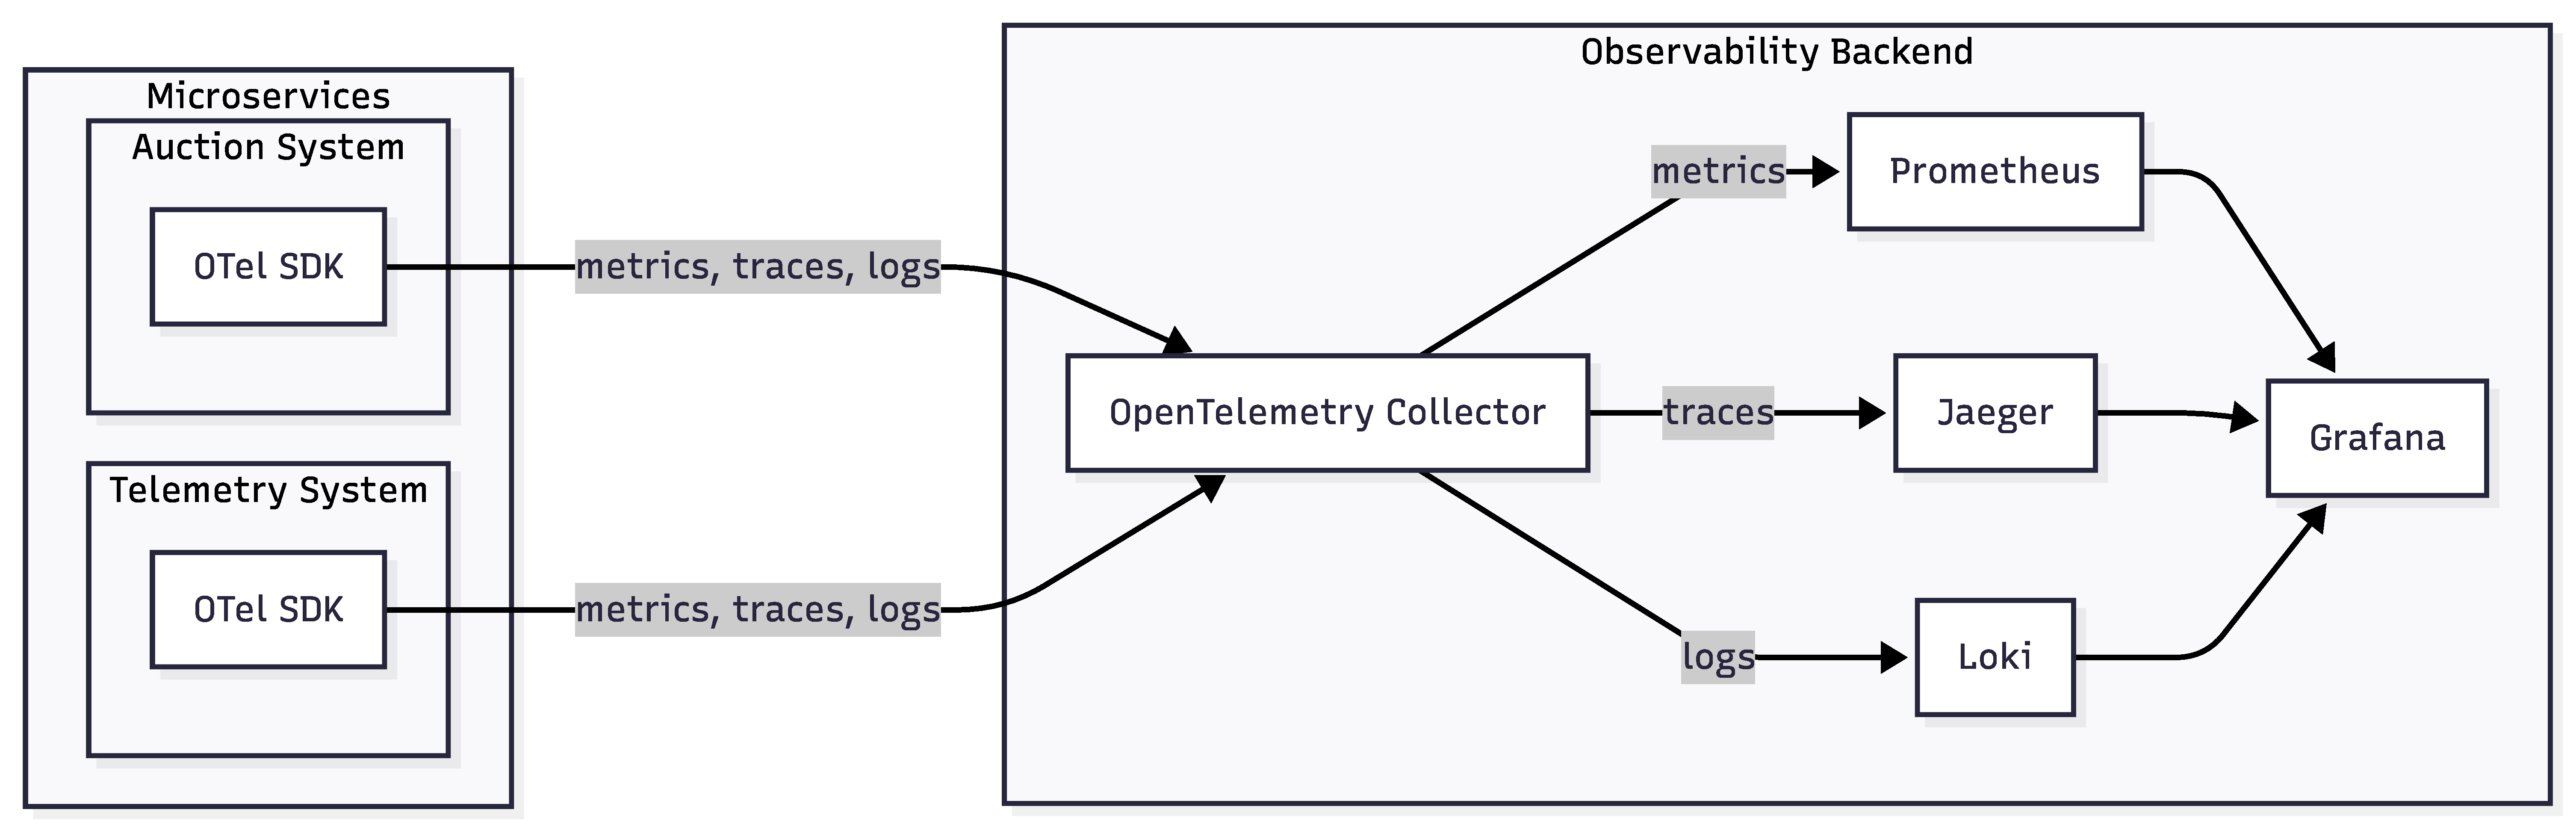
\includegraphics[width=0.95\linewidth]{observability-architecture.pdf}
	}{
		\fbox{\parbox{0.9\linewidth}{\centering
		Mermaid source for this architecture is stored in \texttt{observability-architecture.mmd}. Render it to a PDF and place it in the report folder to include the figure here.
		}}
	}
	\caption{OpenTelemetry-based observability architecture for the global control plane}
	\label{fig:observability-architecture}
\end{figure}

\subsubsection{OpenTelemetry Integration Pattern}

All in-scope microservices are instrumented with OpenTelemetry SDKs and export telemetry through OTLP to a centralized OpenTelemetry Collector. Instrumentation is designed around these conventions \citep{youngLearningOpenTelemetry2023,opentelemetrySpecOTLP}:

\begin{itemize}
	\item domain-prefixed metric instruments (for example, \texttt{ixp.auction.*}, \texttt{ixp.api.*});
	\item stable label sets to avoid excessive time-series cardinality;
	\item explicit units (for example \texttt{kbps}, \texttt{SGD}, \texttt{ms}) for alert consistency;
	\item graceful shutdown flushing to reduce metric loss during rollout and restart events.
\end{itemize}

Metrics are transformed by the collector and Prometheus naming rules (dots to underscores, unit suffixes, and counter \texttt{\_total} suffixes).

\subsubsection{Spans and Distributed Context}

Two foundational concepts underpin distributed tracing: \textbf{spans} and \textbf{context}. Understanding their roles is essential for interpreting the implementation code in Chapter 5.

A \textbf{span} is an atomic unit of work or operation within a service. It has a name, start time, end time, and status (success or failure). Each span may contain semantic attributes (such as operation type, component name, or request ID) that provide meaning without requiring human interpretation of timestamps alone. Spans form a directed acyclic graph: a parent span represents a higher-level operation and may have child spans representing sub-operations or dependency calls. For example, an API Gateway request handler is a parent span, and a call to Atomix for state lookup is a child span.

A \textbf{trace} is the full chain of related spans that together represent one end-to-end unit of work across a system. In practical terms, a trace begins with a root span and then collects all child spans created while the request moves through the API Gateway, Auction Runner, Telemetry Processor, and any dependency calls. This is why a single trace can contain multiple spans: each span records one step in the work chain, while the trace captures the entire causal path from start to finish.

A \textbf{distributed context} (or trace context) is the metadata that flows alongside a request as it propagates across service boundaries. It contains the trace ID (unique identifier for the entire request's journey) and span ID (identifier for the current span), allowing a child service to link its spans back to the parent service's request. Context is typically transmitted in request headers (HTTP, gRPC, or Kafka message headers) so that the observability backend can reconstruct the causal chain even when services are geographically or temporally decoupled \citep{w3cTraceContext,opentelemetryDocsContextPropagation}.

In practical terms, when the API Gateway receives a bid and calls Atomix to check policy constraints, the trace context is extracted at API ingress and a client-side dependency span is recorded around the outbound Atomix call. In this project, Atomix is treated as an external black-box dependency and is not instrumented internally, so traces show only the control-plane service spans plus client-side dependency timing from the caller perspective.

The framework uses context for two distinct purposes:
\begin{itemize}
	\item \textbf{Trace propagation}: preserving the trace ID across service calls so spans can be linked in the observability backend.
	\item \textbf{Timeout and cancellation}: golang contexts carry deadlines and cancellation signals, allowing bounded operations that fail fast if dependencies time out.
\end{itemize}

Both purposes are important: the first enables causal debugging, the second prevents resource exhaustion when upstream services are unavailable.

\subsubsection{Distributed Tracing Design}

Trace instrumentation uses span boundaries at request entry, dependency calls, and asynchronous hand-off points. The objective is to reconstruct end-to-end control-path timing for each interval cycle and identify where latency is introduced.

One important design detail in this project is that bid-ingress tracing and auction-execution tracing do not share a single synchronous call chain. Bid spans are created in request-time API handlers, while auction spans are created later in interval-driven runner execution. Because these spans are produced in different execution contexts, direct parent-child continuity is not always available across the shared-state boundary.

Key tracing design choices are:

\begin{itemize}
\item parent-child span structure across in-scope control-plane services, with client-side dependency spans for external systems;
\item semantic span attributes (operation type, component, and key identifiers such as ingress or egress context where appropriate);
\item span-link based correlation for asynchronous bid write to auction read handoff, using propagated trace context in shared store payloads;
\item consistent propagation of context to preserve causal linkage across services.
\end{itemize}

Traces are exported through the OpenTelemetry Collector to Jaeger, where operators can inspect critical-path delay and dependency bottlenecks.

\subsubsection{Structured Logging Design}

Structured logs are emitted with stable keys (service, operation, error class, and contextual identifiers) so that they can be queried reliably in aggregation backends.

The logging layer focuses on evidence that complements metrics and traces:

\begin{itemize}
\item explicit dependency errors (for example timeout, connection, and unavailable states);
\item state-transition events (for example bid handling outcomes and telemetry publication results);
\item recovery and retry behavior during transient failures.
\end{itemize}

Logs are exported through the collector to Loki, enabling timeline-based correlation with alerts and traces during incident analysis.

\subsubsection{Decoupling Telemetry from Request-Critical Paths}

A critical design principle is that the observability infrastructure itself must not become a source of failure. Per the OpenTelemetry error-handling specification, SDKs must handle their own failures gracefully without destabilizing application logic \citep{opentelemetrySpecErrorHandling}.

The framework implements two core safeguards:

\begin{itemize}
	\item \textbf{SDK error handler registration}: Each service registers a custom error handler that logs SDK failures (exporter unavailability, context propagation errors, metric overflow) without affecting request processing. This allows operators to diagnose observability-stack problems independently from application behavior.
	\item \textbf{Non-blocking telemetry patterns}: Bounded context deadlines, non-blocking metric recording, and defensive error classification (timeout, connection, not found, other) ensure that transient observability-collector unavailability does not propagate as user-facing errors.
\end{itemize}

These patterns ensure that when the observability pipeline itself degrades, the control plane remains operational while the SDK error logs surface the infrastructure problem for remediation.

\subsection{Monitoring and Alerting Architecture}

\subsubsection{Collector and Storage Pipeline}

The telemetry data path is structured as follows:

\begin{enumerate}
	\item Services emit OpenTelemetry Protocol (OTLP) telemetry to the OpenTelemetry Collector.
	\item The collector applies memory-limit and batching processors.
	\item Metrics are exported for Prometheus scraping.
	\item Traces are exported to Jaeger.
	\item Logs are exported to Loki.
	\item Prometheus evaluates alert rules on fixed intervals.
	\item Alertmanager groups, deduplicates, and routes alerts to Telegram.
\end{enumerate}

This centralized pipeline decouples application instrumentation from backend storage and notification concerns while preserving cross-signal correlation.

\subsubsection{Alert Rule Taxonomy}

Alert rules are grouped by failure semantics rather than by component ownership:

\begin{itemize}
	\item \textbf{Availability alerts}: reduced API success rate.
	\item \textbf{Dependency-chain alerts}: increasing Atomix operation errors and near-total failure conditions.
	\item \textbf{Congestion alerts}: sustained p50/p95/p99 latency elevation on critical operations.
	\item \textbf{Telemetry continuity alerts}: low or absent flow publication despite expected system activity.
\end{itemize}

This taxonomy improves operator triage by reflecting likely incident phases: early slowdown, partial failure, then widespread service impact. In practice, metric alerts trigger first, traces identify delayed segments, and logs provide root-cause evidence.

\subsubsection{Severity Mapping and Notification Policy}

To reduce alert fatigue while preserving responsiveness, rule severities are staged:

\begin{itemize}
	\item \textbf{Warning}: early anomalous behavior that may self-recover but should be watched.
	\item \textbf{Critical}: probable service impact requiring prompt intervention.
\end{itemize}

Alertmanager routes notifications to Telegram with labels and annotations describing likely cause, affected path, and suggested first checks.

\subsection{Summary}

The resulting framework combines metric semantics, distributed tracing, structured logging, rule design, and operator workflow into one control-plane observability system. Its design emphasis is early warning for soft failures and actionable incident triage, preparing the ground for the implementation details and evaluation scenarios in the next chapters.
